\documentclass[12pt, letterpaper, twoside]{article}
%%%%%%%%%%%%%%%%%%%%%%%%
% Imports
%%%%%%%%%%%%%%%%%%%%%%%%
\usepackage[utf8]{inputenc}
\usepackage[acronyms]{glossaries}
\usepackage{graphicx}
\usepackage{biblatex}

%%%%%%%%%%%%%%%%%%%%%%%%
% Metadata
%%%%%%%%%%%%%%%%%%%%%%%%
\title{EWT summary}
\author{Ernesto Casablanca}
\date{\today}
\graphicspath{ {./img/} }

%%%%%%%%%%%%%%%%%%%%%%%%
% Glossary
%%%%%%%%%%%%%%%%%%%%%%%%
% \makeglossaries
\newacronym{did}{DID}{Decentralized IDentifiers}
\newacronym{der}{DER}{Distributed Energy Resource}
\newacronym{dsm}{DSM}{Demand Side Management}
\newacronym{irec}{I-REC}{International Renewable Energy Certificate}
\newacronym{poa}{POA}{Proof of Authority}
\newacronym{evm}{EVM}{Ethereum Virtual Machine}
\newacronym{erc}{ERC}{Ethereum Request for Comment}
\newacronym{ewns}{EWNS}{Energy Web Name Service}
\newacronym{ewc}{EWC}{Energy Web Chain}
\newacronym{eac}{EAC}{energy Attribute Certificate}

%%%%%%%%%%%%%%%%%%%%%%%%
% References
%%%%%%%%%%%%%%%%%%%%%%%%
\addbibresource{resources.bib} %Import the bibliography file

%%%%%%%%%%%%%%%%%%%%%%%%
% Init document
%%%%%%%%%%%%%%%%%%%%%%%%
\begin{document}

% \begin{titlepage}
%     \maketitle
% \end{titlepage}

\tableofcontents

\newpage

\begin{abstract}
    Questo è un breve riassunto per punti che contiene le mie prime impressioni
    a proposito del progetto Energy Web
\end{abstract}

\section{Problemi da risolvere}

\subsection{Ammodernamento della gestione della rete elettrica}
In passato, una gestione centralizzata della rete elettrica era più che ragionevole.
I grandi operatori elettrici erano anche quelli che producevano anche la quasi totalità dell'energia, avendo a disposizione i mezzi per realizzare impianti costosi e complessi.
La situazione odierna, tuttavia, è diversa.\\
Negli anni abbiamo assistito ad una riduzione progressiva del costo degli impianti per la produzione di energia rinnovabile.
Ne è conseguita una diffusione sempre più capillare di piccoli produttori di energia elettrica, che attraverso impianti, spesso domestici, sono in grado di offrire un contributo alla rete.\\
La gestione di queste piccole realtà, però, mal si sposa con l'attuale struttura centralizzata, e impone un cambio di paradigma verso un'architettura distribuita, che metta in contatto produttore e consumatore.

\begin{figure}[h]
    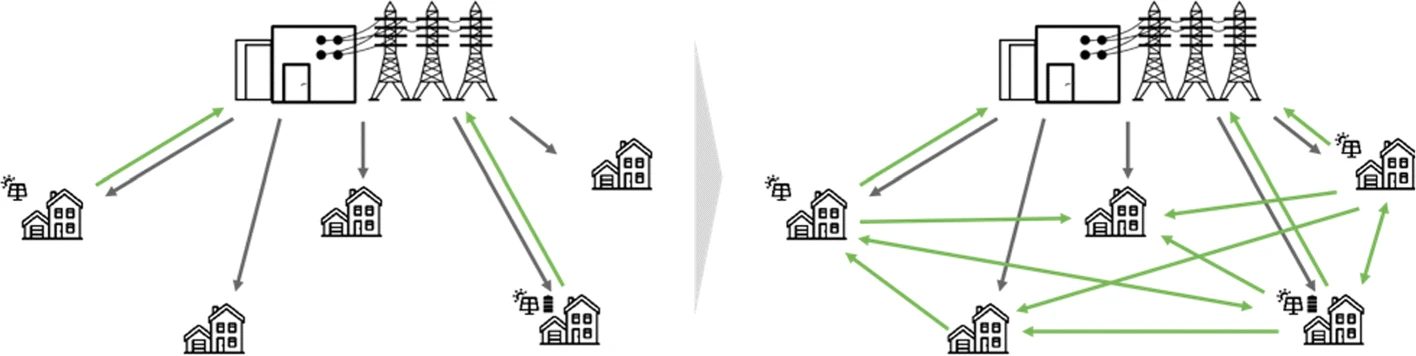
\includegraphics[width=9cm]{p2pgrid}
    \centering
    \label{p2pgrid}
    \caption{Da rete da centralizzata a p2p \cite{img:p2pgrid}}
\end{figure}

\subsection{Certificazione di sostenibilità ambientale}
Dopo anni di scarsa sensibilità sull'argomento "sostenibilità ambientale", negli ultimi anni abbiamo assistito ad un'inversione di rotta.
Man mano che gli effetti della combustione fossile sull'ambiente diventano sempre più evidenti e pericolosi, si manifesta sempre più spesso nei consumatori la volontà di acquistare energia da fonti rinnovabili.\\
C'è quindi la necessità di creare un equivalente di un'etichetta di identificazione per l'energia, permettendo all'utente di scegliere di acquistare la propria energia da un produttore che abbia una certificazione come l'"\gls{irec}"

\newpage

\section{Implementazione}
Il cuore del progetto di Energy Web è EW-DOS, un'infrastruttura open-source, pubblica e digitale.
L'intero sistema è costituito da tre macro componenti, ognuno con uno scopo specifico:
\begin{itemize}
    \item Trust - \gls{ewc}
    \item Utility - Servizi e astrazioni sopra la blockchain
    \item Toolkit - Frameworks per la costruzione di applicazioni
\end{itemize}

\begin{figure}[h]
    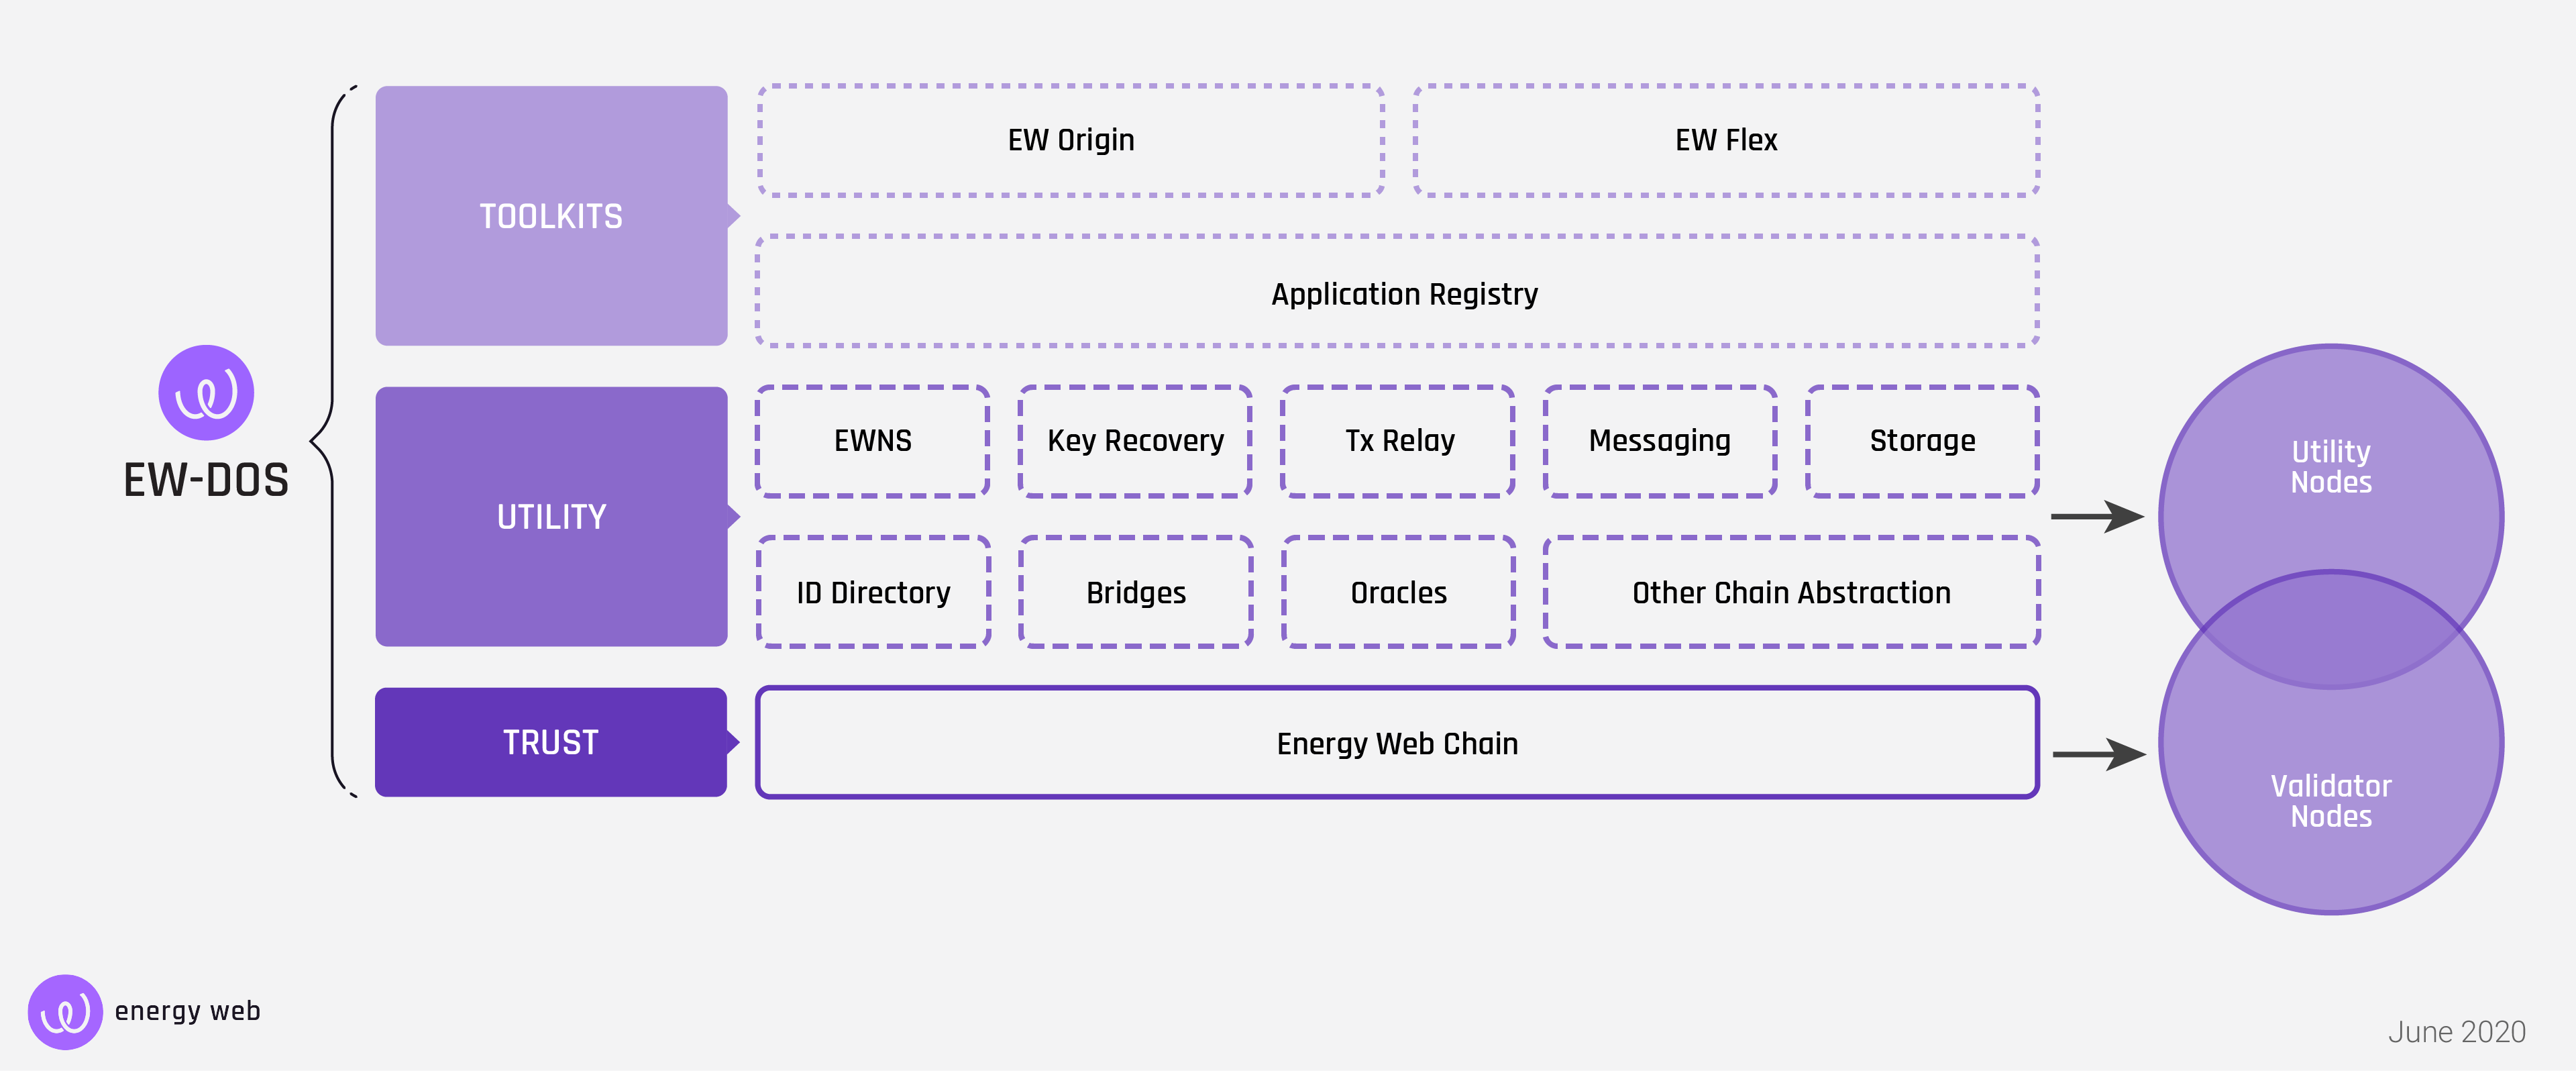
\includegraphics[width=13cm]{ew-dos}
    \centering
    \label{ew-dos}
    \caption{Visualizzazione della struttura di EW-DOS \cite{img:ew-dos}}
\end{figure}

\subsection{Trust}
Il ruolo principale della \gls{ewc} è quello di assicurare che ci sia consenso sui dati e che tutte le applicazioni e gli smart contracts si comportino in maniera deterministica.\\
Si basa sulla \gls{evm} e consente la creazione di smart contract, rispettando tutti gli \gls{erc}.\\
È presente anche una test-net, chiamata Volta, usata per testare i progetti e le applicazioni prima di lanciare sulla main-net.

\subsubsection{Algoritmo di consenso}
L'algoritmo di consenso è \gls{poa}, basato sul protocollo AuRA\cite{art:aura}. \\
Vi sono dei nodi specifici nella rete che hanno il ruolo di validatori, e sono gli unici nodi in grado di validare nuovi blocchi ed aggiungerli alla blockchain.
Questi nodi appartengono alle organizzazioni partner di Energy Web. Oggi, \today, sono 44, e il loro contributo può essere visto in diretta al link https://validators.energyweb.org/.\\
Sebbene venga sacrificata una decentralizzazione assoluta, il vantaggio di questo protocollo si manifesta in un throughput molto maggiore rispetto ad altre blockchain.
Al momento il throughput è circa da 2 a 3 volte quello di Ethereum, ma in condizioni ideali può esserlo di 7.5 volte\cite{art:ew-dos}.

\subsubsection{EWT token}
Il token usato nella Energy Web blockchain si chiama EWT.
Vengono utilizzati per pagare le transazioni e tutti gli altri servizi dell'EW-DOS.
A causa delle grande specificità di utilizzo della rete, le tariffe sono generalmente molto basse e vanno dallo $0.00001$ allo $000000.1$ di EWT.

\subsection{Utility}
L'utility layer è composto da un insieme di servizi basati sulla \gls{ewc} che hanno lo scopo di rendere quanto più accessibile e invitante possibile l'intera infrastruttura per gli sviluppatori.\\
Tutti i servizi vengono pagati in EWT.
Vengono individuate 3 ampie categorie di servizi:
\begin{itemize}
    \item Esperienza dell'utente finale
    \item Interoperabilità Multipiattaforma
    \item Performance delle applicazioni
\end{itemize}

\subsubsection{Esperienza dell'utente finale}
\begin{itemize}
    \item \gls{ewns} - Stesso principio di un DNS, associa domini ad indirizzi sulla blockchain
    \item DID Key Recovery - Permette il recupero della propria DID nel caso si fosse persa la chiave privata
    \item Transaction Relay - Servizio che fa da intermediario fra un cliente e la blockchain, nascondendo l'utilizzo della stessa
\end{itemize}

\subsubsection{Interoperabilità Multipiattaforma}
\begin{itemize}
    \item Bridges - Consente il trasferimento di token fra blockchain diverse
    \item Oracles - Particolari nodi che è possibile consultare con il protocollo Chainlink per ricevere dati di eventi esterni alla blockchain
\end{itemize}

\subsubsection{Performance delle applicazioni}
\begin{itemize}
    \item Identity Directory - Smart contract che contiene tutti le \gls{did}
    \item Messaging - Un sistema di messaggistica che sfrutta le \gls{did} per assicurare validità ed autenticità dei messaggi
    \item Storage - Memoria sulla blockchain
\end{itemize}

\newpage

\section{Toolkit}
Framework ed applicazioni di esempio per realizzare applicazioni decentralizzate su EW-DOS. \\

\subsection{Application Registry}
Registro di \gls{did} che soddisfano una certa condizione, come ad esempio la località geografica o il possesso di una certa qualifica.\\
Ogni applicazione distribuita deve fare riferimento ad un Application Registry, che può essere riutilizzato in più applicazioni.

\subsection{EW origin}
Framework per sviluppare applicazioni che supportino il tracciamento, la trasmissione e il conferimento di \gls{eac} secondo gli standard industriali.

\subsection{EW flex}
Software open source per la gestione dei \gls{der} e le operazioni che li coinvolgono, permettendone una facile connessione alla rete, sottoponendo le offerte ad un operatore autorizzato.

\newpage

\section{Provati con mano}
Elenco dei servizi offerti da Energy Web che ho provato con mano e sui quali 

\subsection{\gls{ewns}}
Servizio simil-DNS offerto da Energy Web. Lo si trova all'indirizzo https://ens.energyweb.org/.\\
Permette di cercare gli indirizzi sulla blockchain utilizzando un dominio, nonchè di registrare un proprio dominio.\\
Può essere integrato in altre applicazioni per risolvere i domini, rendendo molti processi più user-friendly.

\subsection{Switchboard}
Applicazione che promette di diventare il cuore pulsante dell'intero sistema. Lo si trova all'indirizzo https://volta-switchboard.energyweb.org/ \\
Si tratta di una GUI intuitiva che premette:
\begin{itemize}
    \item la gestione di \gls{did}, compresa la loro categorizzazione in base alle certificazioni che possiedono
    \item la gestione degli asset fisici in proprio possesso, con la possibilità di iscriverli in varie dApps, ammesso che soddisfino le caratteristiche richieste
    \item l'utilizzo di un app store per trovare altre dApps sulla blockchain
    \item iscriversi a vari servizi come quello della messaggistica e della gestione delle chiavi
\end{itemize}
Proprio perchè si tratta di un prodotto molto ambizioso, la maggior parte delle funzionalità promesse non siano state implementate.

\subsection{Smart contract}
È possibile effettuare il deploy di smart contract sulla testnet Volta, come su qualsiasi altra blockchain derivata da Ethereum.

\newpage

\section{Conclusione}
Energy Web è senza dubbio un progetto con un buon potenziale. \\
Essendo portato avanti da persone che conoscono bene il settore energetico e le sue problematiche, non cerca di fare il passo più lungo della gamba con una decentralizzazione totale, ma piuttosto si accontenta di decentralizzare quanto più possibile in piccoli step progressivi. \\
Questo anche con lo scopo di rendere l'intera piattaforma quanto più appetibile ai possibili partner, in numero che appare sempre in crescita. \\
C'è ovviamente anche un focus per quanto riguarda il lato utente.
Questo si traduce sia in un incentivo all'acquisto consapevole di energia verde certificata, sia in un'offerta di DApp che possano sfruttare le peculiarità dell'EW-DOS.

\begin{figure}[h]
    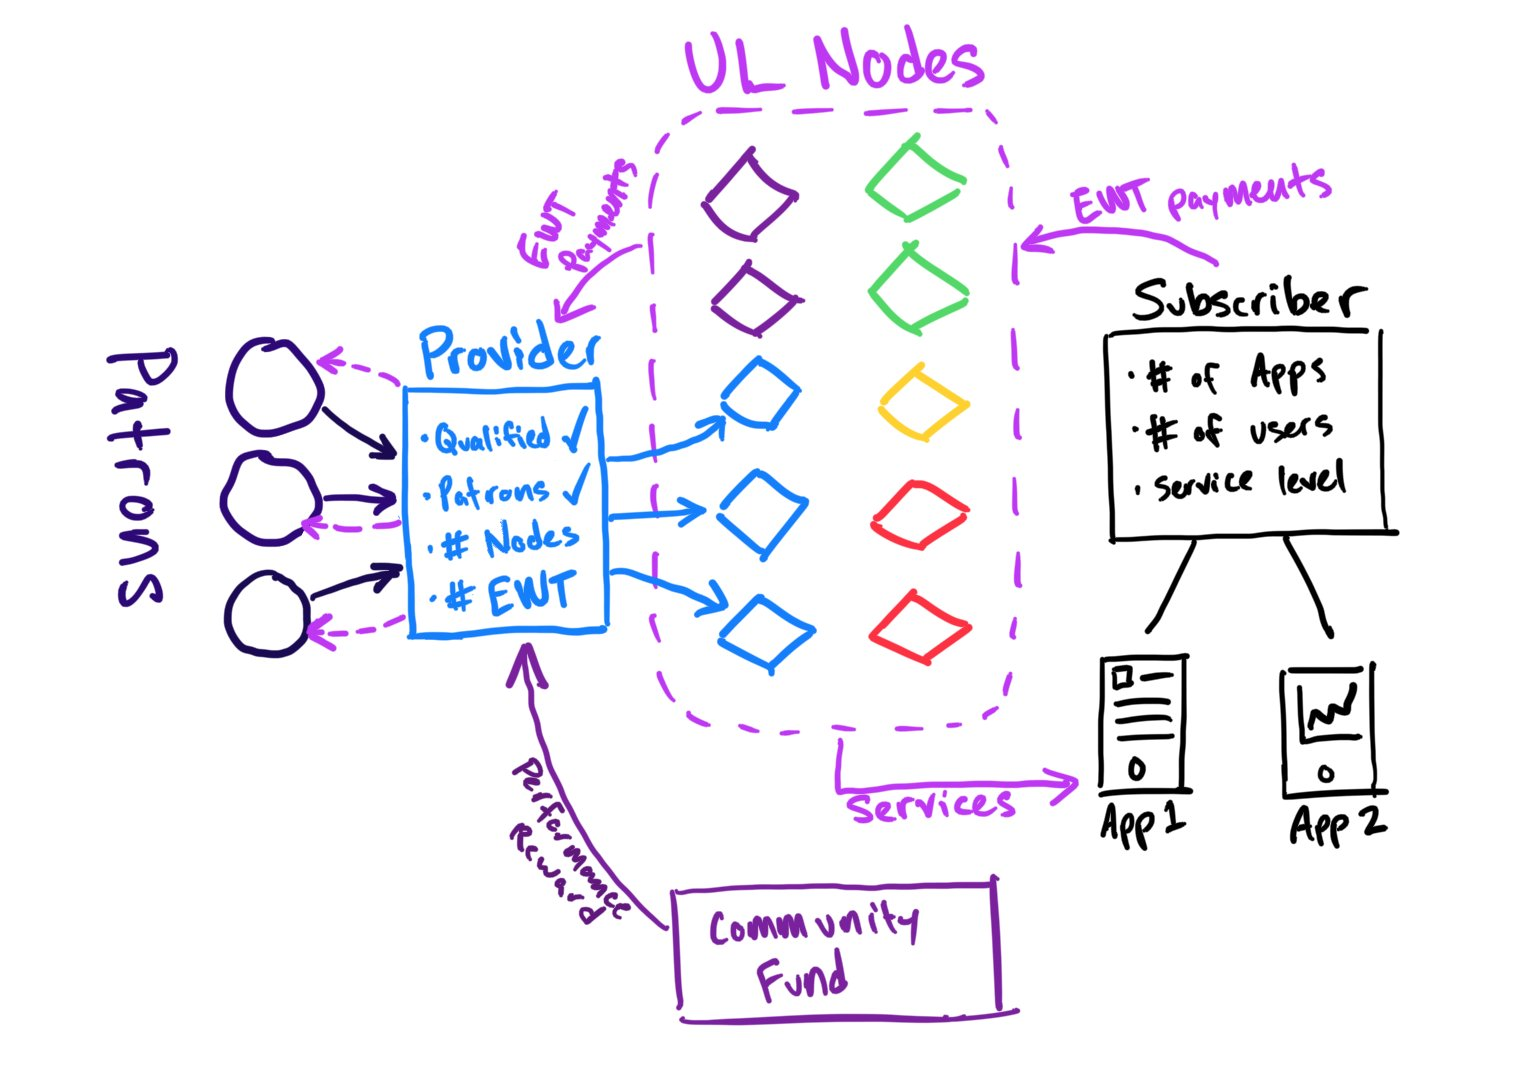
\includegraphics[width=13cm]{ew-staking}
    \centering
    \label{ew-staking}
    \caption{Schema della struttura di EW-DOS con staking \cite{art:ew-staking}}
\end{figure}

\newpage

\printbibliography
\end{document}
